
\chapter{4\(f\)光学系统}
\section{数学概念说明}

定义矩形函数、矩形孔特征衍射函数(即sinc函数)、圆孔函数、圆孔衍射特征函数如下
\begin{align*}
	\Pi(\xi) =
	\begin{cases}
		1, & |\xi| \leq \frac{1}{2} \\
		0, & |\xi| > \frac{1}{2}
	\end{cases},
	\quad \sinc(x)=\frac{\sin x}{x},\quad
	\text{circ}(\xi) =
	\begin{cases}
		1, & \xi \leq 1 \\
		0, & \xi > 1
	\end{cases},
	\quad
	A(\xi) = \frac{2 J_1(\xi)}{\xi}.
\end{align*}
其中\(J_1(\xi)\)是1阶贝塞尔函数.相关傅里叶变换公式为
\begin{align*}
	&\int_{-\infty}^{\infty} \Pi\left(\frac{x}{w}\right) e^{-i 2 \pi f x} dx = w \cdot \sinc(\pi w f)\\
	&\iint_{-\infty}^{\infty} \text{circ}\left(\frac{\sqrt{x^2 + y^2}}{R}\right) e^{-i 2 \pi (f_x x + f_y y)} dxdy = R^2 \cdot A\left(2 \pi R \sqrt{f_x^2 + f_y^2}\right).
\end{align*}

当方孔的边长等于圆孔的直径时，两者的频谱图如下.用肉眼观察，两者的中心谱斑区域形状相差不大，主要差异在于次极大的分布：方孔的次极大沿边长方向“十”字延展，圆孔的次极大则以同心圆状向外延展.然而，由于中心谱斑光强过大，这种次极大分布的差异在实验中较难分辨.

\begin{figure}[htbp]
	\centering
	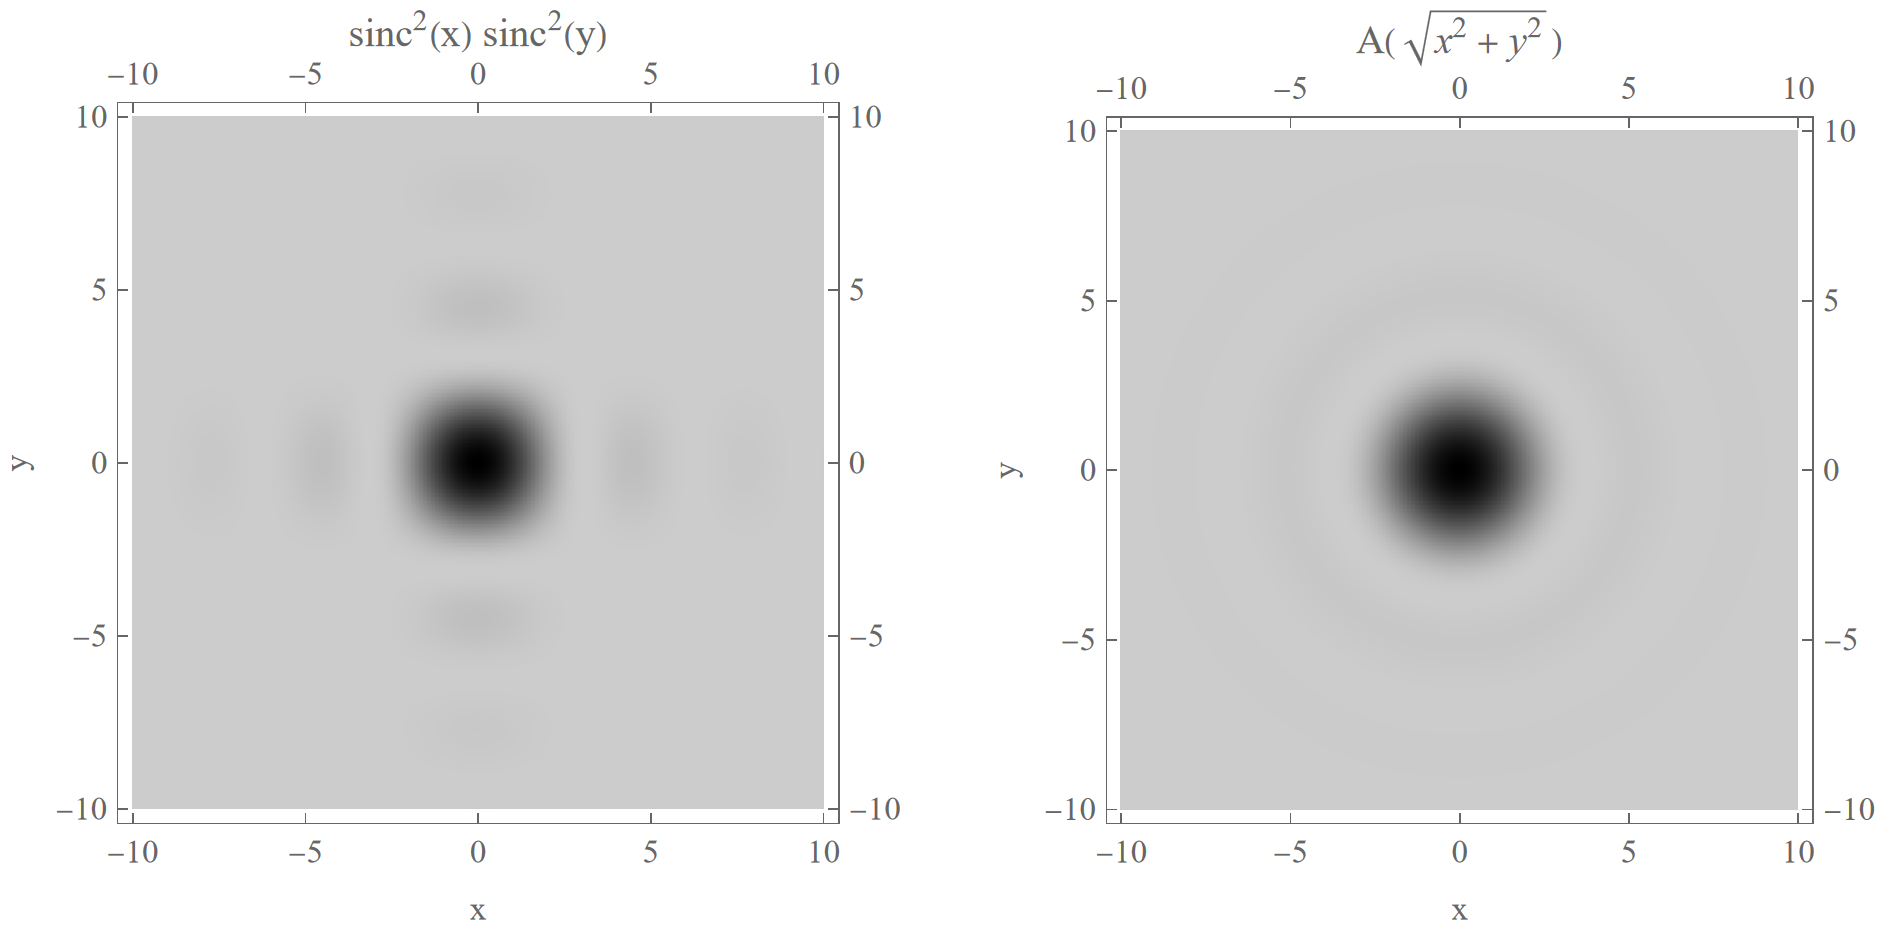
\includegraphics[width=0.5\textwidth]{fourier_optics_4f_fig/square_and_circular_aperture_spectrum_comparison_plot.png}
	\caption{方孔圆孔频谱比较图}
	\label{fig:square_vs_circular_aperture_spectrum}
\end{figure}

定义一维卷积为（更高的维数同理）
\begin{align*}
	(f * g)(\xi) = \int_{-\infty}^{\infty} f(\xi - \xi') g(\xi') d\xi'.
\end{align*}

不难验证
\begin{align*}
	\int_{-\infty}^{\infty} (f * g)(x) e^{i k x} dx = \left( \int_{-\infty}^{\infty} f(x) e^{i k x} dx \right) \cdot \left( \int_{-\infty}^{\infty} g(x') e^{i k x'} dx' \right).
\end{align*}
\begin{align*}
	\int_{-\infty}^{\infty} f(x) g(x) e^{i k x} dx = \frac{1}{2\pi} \left( \int_{-\infty}^{\infty} f(x) e^{i k x} dx \right) * \left( \int_{-\infty}^{\infty} g(x') e^{i k x'} dx' \right).
\end{align*}

\section{4\(f\)系统的基本结论.}

\begin{figure}[htbp]
	\centering
	
\includegraphics[width=0.75\textwidth]{fourier_optics_4f_fig/four_f_system_schematic_diagram.png}
	\caption{4\(f\)系统示意图}
	\label{fig:four_f_system}
\end{figure}
4\(f\)系统光路如\cref{fig:four_f_system}.记物面振幅分布 \( U_o(x, y) \) ，对球面波因子进行傍轴近似、忽略轴向转播因子，得频谱面振幅分布：

\begin{align*}
	U_f(x_f, y_f) =\frac{1}{\lambda f} \iint U_o(x, y) e^{-i \frac{2\pi}{\lambda f} (x x_f + y y_f)} dx dy
\end{align*}
其中 \( (x_f, y_f) \) 是频谱面的实际空间坐标.

可见，频谱面的振幅分布恰体现了物面振幅分布的傅里叶变换，相应空间频率为
\begin{align*}
	f_x=\frac{x_f}{\lambda f},\quad f_y=\frac{y_f}{\lambda f}
\end{align*}

以空间波矢\(\vb{\kappa}=2\pi(f_x\uv{x}+f_y\uv{y})\)为变量，频谱面的振幅函数可简写为
\begin{align*}
	\tilde{U}_f(\vb{\kappa})=U_f(\lambda f f_x,\lambda f f_y)=\frac{1}{\lambda f} \int U_o(\vb{r}) e^{-i \vb{\kappa}\cdot\vb{r}} d\vb{r}
\end{align*}

在频谱面上，记滤波器的透过率分布为 \(H(x_f, y_f)\)，则滤波后的频谱为：
\begin{align*}
	U_f'(x_f, y_f) = U_f(x_f, y_f) \cdot H(x_f, y_f)
\end{align*}

经过第二个变换透镜，得到像面振幅分布为：
\begin{align*}
	U_P(x, y) = \frac{1}{\lambda f}\iint U_f'(x_f, y_f) e^{i \frac{2\pi}{\lambda f} (x x_f + y y_f)} dx_f dy_f= \frac{1}{\lambda f}\iint U_o(\xi, \eta) h(x - \xi, y - \eta) d\xi d\eta.
\end{align*}
其中
\begin{align*}
	h(x, y) = \frac{1}{\lambda f}\iint H(x_f, y_f) e^{i \frac{2\pi}{\lambda f} (x x_f + y y_f)} dx_f dy_f
\end{align*}

实验中，可直接测量频谱面上滤波器后的光强分布和像面的光强分布：
\begin{align*}
	&I_f'(x_f, y_f) = |U_f'(x_f, y_f)|^2 = |U_f(x_f, y_f) \cdot H(x_f, y_f)|^2\\
	&I_P(x, y) = |U_P(x, y)|^2 = \left|\frac{1}{\lambda f} (U_o*h)(x,y)\right|^2.
\end{align*}

\section{频谱面的振幅分布}
\section{单孔振幅}
频谱面上的振幅分布体现了物面振幅分布的傅里叶变换，将频谱面的空间坐标除以常数因子\(\lambda f\)便是相应的空间频率.以空间频率对应的波矢来表示，即(记\(\vb{r}=x\uv{x}+y\uv{y}\))
\begin{align*}
	\tilde{U}_f(\vb{\kappa})=U_f(\lambda f f_x,\lambda f f_y)=\frac{1}{\lambda f} \int U_o(\vb{r}) e^{-i \vb{\kappa}\cdot\vb{r}} d\vb{r}
\end{align*}

当物为较规则的几何形状时，该式可以解析计算，相应频谱图像可以解析分析.下考虑均匀平面波入射，物为某种形状的理想孔的规则密排.

\textbf{先计算每个单元的频谱函数}

\begin{exbox}
	边长为 \(w_1, w_2\) 矩形孔
	\begin{align*}
		U_o^{\text{unit}}(x, y) = \Pi\left( \frac{x}{w_1} \right) \Pi\left( \frac{y}{w_2} \right), \quad \tilde{U}_f^{\text{unit}}(\vb{\kappa}) = \frac{w_1 w_2}{\lambda f} \sinc\left( \frac{\kappa_x w_1}{2} \right) \sinc\left( \frac{\kappa_y w_2}{2} \right)
	\end{align*}
\end{exbox}

\begin{exbox}
	半径为 \(R\) 的圆孔
	\begin{align*}
		U_o^{\text{unit}}(x, y) = \text{circ}\left( \frac{\sqrt{x^2 + y^2}}{R} \right), \quad \tilde{U}_f^{\text{unit}}(\vb{\kappa}) = \frac{\pi R^2}{\lambda f} A(\kappa R)
	\end{align*}
\end{exbox}

\begin{exbox}
	\(N\)边形孔

	将\(N\)边形的顶点逆时针编为0至\(N-1\) (\(N\)号等价于1号)，记 \(\vb{L}_j\) 为\(j\)号顶点指向\(j + 1\)号顶点的矢径，记 \(\vb{R}_j\) 为该边中点的位矢.用二维高斯定理不难证明(\(D\)为\(N\)边形的区域)
	\begin{align*}
		\tilde{U}_f^{\text{unit}}(\vb{\kappa}) = \frac{1}{\lambda f} \iint_D e^{-i \vb{\kappa} \cdot \vb{r}} d^2 r= -\frac{i}{\lambda f} \sum_{j=0}^{N-1} \frac{\vb{L}_j \cdot \uv{x}}{\vb{\kappa} \cdot \uv{y}} e^{-i \vb{\kappa} \cdot \vb{R}_j} \sinc\left( \frac{\vb{\kappa} \cdot \vb{L}_j}{2} \right) = \frac{i}{\lambda f} \sum_{j=0}^{N-1} \frac{\vb{L}_j \cdot \uv{y}}{\vb{\kappa} \cdot \uv{x}} e^{-i \vb{\kappa} \cdot \vb{R}_j} \sinc\left( \frac{\vb{\kappa} \cdot \vb{L}_j}{2} \right).
	\end{align*}
\end{exbox}

\begin{exbox}
	底边长\(2b\)、高\(h\)的等腰三角形孔

	将原点取在底边高线的中点处，使得三个顶点的坐标为 \((\pm b, -h/2),\,(0, h/2)\)，运用\(N\)边形孔的结论，易得频谱面的振幅为
	\begin{align*}
		\tilde{U}_f^{\text{unit}}(\vb{\kappa}) = -\frac{i h}{\lambda f \kappa_x} \left( e^{i b \kappa_x/2} \sinc\left(\frac{b \kappa_x + h \kappa_y}{2}\right) -  e^{-i b \kappa_x/2} \sinc\left(\frac{b \kappa_x - h \kappa_y}{2}\right) \right).
	\end{align*}
\end{exbox}

\section{单孔密排振幅}

取线性无关矢量 \(\vb{a}_1, \vb{a}_2\)，使 \((m, n)\) 号孔相对基点 \(\vb{r}\) 处孔的位矢为 \(\vb{R}_{mn} = m \vb{a}_1 + n \vb{a}_2\)；

记 \(A_c = |\vb{a}_1 \times \vb{a}_2|\)，取如下倒格矢，并记 \(\vb{G}_{hl} = h \vb{b}_1 + l \vb{b}_2\,(m,\,n,\,h,\,l\in \mathbb{Z})\)
\begin{align*}
	\vb{b}_i \cdot \vb{a}_j = 2\pi \delta_{ij}, \quad \vb{b}_1 = \frac{2\pi}{A_c} (a_{2y}, -a_{2x}), \quad \vb{b}_2 = \frac{2\pi}{A_c} (-a_{1y}, a_{1x})
\end{align*}


进而，梳状函数可以在某个孔单元内做傅里叶展开为
\begin{align*}
	\amalg(\vb{r}) = \sum_{m=-\infty}^{\infty} \sum_{n=-\infty}^{\infty} \delta(\vb{r} - \vb{R}_{mn}) = \sum_{h=-\infty}^{\infty} \sum_{l=-\infty}^{\infty} \frac{1}{A_c} e^{i \vb{G}_{hl} \cdot \vb{r}}.
\end{align*}

实际上的物不可能无限大，其只有某一区域\(D\)内有孔.引入窗函数
\begin{align*}
	W(\vb{r}) =
	\begin{cases}
		1, & \vb{r} \in D \\
		0, & \text{else}
	\end{cases}.
\end{align*}

则频谱面的振幅为
\begin{align*}
	\tilde{U}_f(\vb{\kappa}) = \frac{1}{\lambda f} \int U_o(\vb{r}) * (W(\vb{r}) \amalg(\vb{r})) e^{-i \vb{\kappa} \cdot \vb{r}} d\vb{r} = \tilde{U}_f^{\text{unit}}(\vb{\kappa}) \sum_{h=-\infty}^{\infty} \sum_{l=-\infty}^{\infty} \frac{1}{A_c} \tilde{W}(\vb{\kappa} - \vb{G}_{hl}).
\end{align*}
其中 \(\tilde{U}_f^{\text{unit}}(\vb{\kappa})\) 代表单个该形状的孔的频谱面振幅分布，\(\tilde{W}(\vb{\kappa})\) 是 \(W(\vb{r})\) 的傅里叶变换

\begin{align*}
	\tilde{W}(\vb{\kappa}) = \int W(\vb{r}) e^{-i \vb{\kappa} \cdot \vb{r}} d\vb{r}.
\end{align*}

对于两边矢量为 \(L_1 \uv{u}_1, L_2 \uv{u}_2\) 的平行四边形窗口
\begin{align*}
	W(\vb{r}) &= \Pi\left( \frac{\vb{r} \cdot \uv{u}_1}{L_1} \right) \Pi\left( \frac{\vb{r} \cdot \uv{u}_2}{L_2} \right), \quad \tilde{W}(\vb{\kappa}) = L_1 L_2 \sinc\left( \frac{\vb{\kappa} \cdot \uv{u}_1}{2} L_1 \right) \sinc\left( \frac{\vb{\kappa} \cdot \uv{u}_2}{2} L_2 \right)\\
	\tilde{U}_f(\vb{\kappa}) &= \tilde{U}_f^{\text{unit}}(\vb{\kappa}) \frac{L_1 L_2}{A_c} \sum_{h=-\infty}^{\infty} \sum_{l=-\infty}^{\infty} \sinc\left( \frac{(\vb{\kappa} - \vb{G}_{hl}) \cdot \uv{u}_1}{2} L_1 \right) \sinc\left( \frac{(\vb{\kappa} - \vb{G}_{hl}) \cdot \uv{u}_2}{2} L_2 \right).
\end{align*}

容易看到，极大斑点位于
\begin{align*}
	(\vb{\kappa} - \vb{G}_{hl}) \cdot \uv{u}_1=0,\quad (\vb{\kappa} - \vb{G}_{hl}) \cdot \uv{u}_2=0
\end{align*}
斑点的全平面强度分布由单元的强度分布函数调制.

最常见的，取一个矩形窗口，\(\uv{u}_1=\uv{x},\,\uv{u}_2=\uv{y}\).考虑如下立方密排、六角密排情形.

\begin{exbox}
	对于立方密排
	\begin{align*}
		\vb{a}_1 = d \uv{x}, \quad \vb{a}_2 = d \uv{y}, \quad A_c = d^2, \quad \vb{G}_{hl} = \frac{2\pi}{d} (h \uv{x} + l \uv{y}).
	\end{align*}
	\begin{align*}
		\tilde{U}_f(\vb{\kappa}) = \tilde{U}_f^{\text{unit}}(\vb{\kappa}) \frac{L^2}{d^2} \sum_{h=-\infty}^{\infty} \sum_{l=-\infty}^{\infty} \sinc\left( \frac{\kappa_x L_1}{2} - \pi h \frac{L_1}{d} \right) \sinc\left( \frac{\kappa_y L_2}{2} - \pi l \frac{L_2}{d} \right)
	\end{align*}
	极大斑点位于
	\begin{align*}
		\kappa_x=\frac{2\pi h}{d},\quad \kappa_y=\frac{2\pi l}{d}
	\end{align*}
\end{exbox}

\begin{exbox}
	对于六角密排
	\begin{align*}
		\vb{a}_1 = d \uv{x}, \quad \vb{a}_2 = d \left( \frac{1}{2} \uv{x} + \frac{\sqrt{3}}{2} \uv{y} \right), \quad A_c = \frac{\sqrt{3}}{2} d^2, \quad \vb{G}_{hl} = \frac{2\pi}{d} \left( h \uv{x} + \frac{1}{\sqrt{3}} (-h + 2l) \uv{y} \right)
	\end{align*}
	\begin{align*}
		\tilde{U}_f(\vb{\kappa}) = \tilde{U}_f^{\text{unit}}(\vb{\kappa}) \frac{2 L^2}{\sqrt{3} d^2} \sum_{h=-\infty}^{\infty} \sum_{l=-\infty}^{\infty} \sinc\left( \frac{\kappa_x L_1}{2} - \pi h \frac{L_1}{d} \right) \sinc\left( \frac{\kappa_y L_2}{2} - \frac{\pi}{\sqrt{3}} (-h + 2l) \frac{L_2}{d} \right)
	\end{align*}
	极大斑点位于
	\begin{align*}
		\kappa_x=\frac{2\pi h}{d},\quad \kappa_y=\frac{2\pi(-h+2l)}{\sqrt{3}d}
	\end{align*}
\end{exbox}

\section{频谱模拟}
最后，用mathematica的离散傅里叶变换功能模拟频谱面（如\cref{fig:object_and_spectrum_plane}）.
取\(\lambda=632.8\text{nm},\,f=250\text{mm}\).各类型孔/屏理想化为全透/全不透，几何参数如下：

- 物面均限制在4mm\(\times\)4mm的正方窗口内.

- 长方孔长为0.7mm、宽为0.3mm，双长方孔中心间距0.5mm.

- 五角星孔外接圆半径0.8mm.

- 等腰三角形底边为1mm、高为1.3mm.

- 圆孔半径为0.3mm，双圆孔中心间距0.8mm.

- 单个缝长为3mm、宽为0.25mm，中心间距0.4mm.

- 立方或六角密排方孔边长0.25mm、中心间距0.3mm.

- 立方或六角密排圆孔半径0.15mm、中心间距0.36mm.

- 十字架臂长1.6mm、臂宽0.2mm.

- 二维光栅横纵周期均为0.21mm、占空比30\(\%\).


\begin{figure}[htbp]
	\centering

	\begin{subfigure}[b]{0.49\textwidth}
		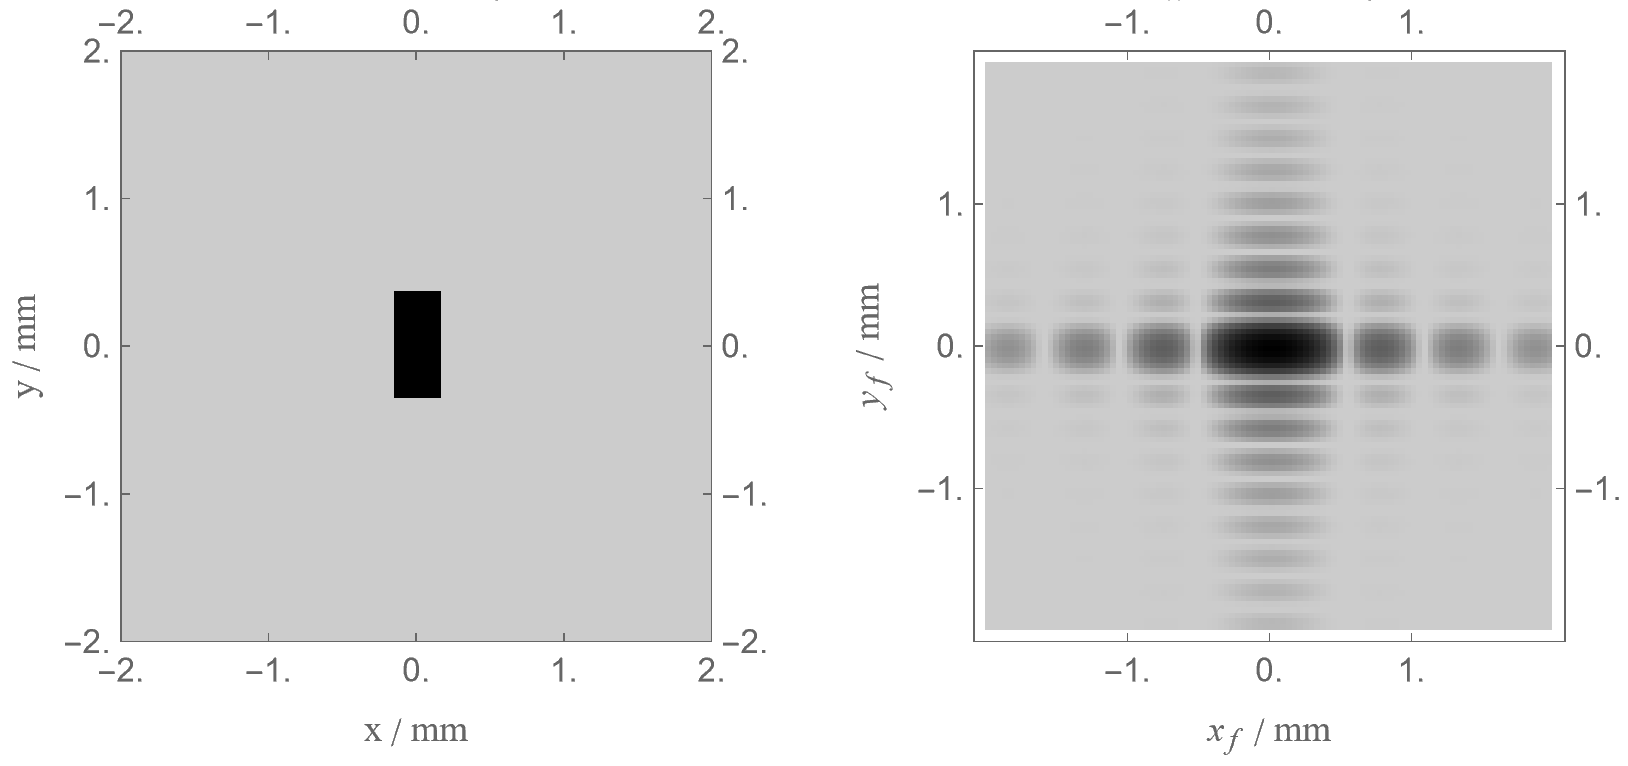
\includegraphics[width=\textwidth]{fourier_optics_4f_fig/single_rectangular_aperture.png}
		\caption{单长方孔}
		\label{fig:object_spectrum_rect_single}
		\label{fig:rect_single}
	\end{subfigure}
	\hfill
	\begin{subfigure}[b]{0.49\textwidth}
		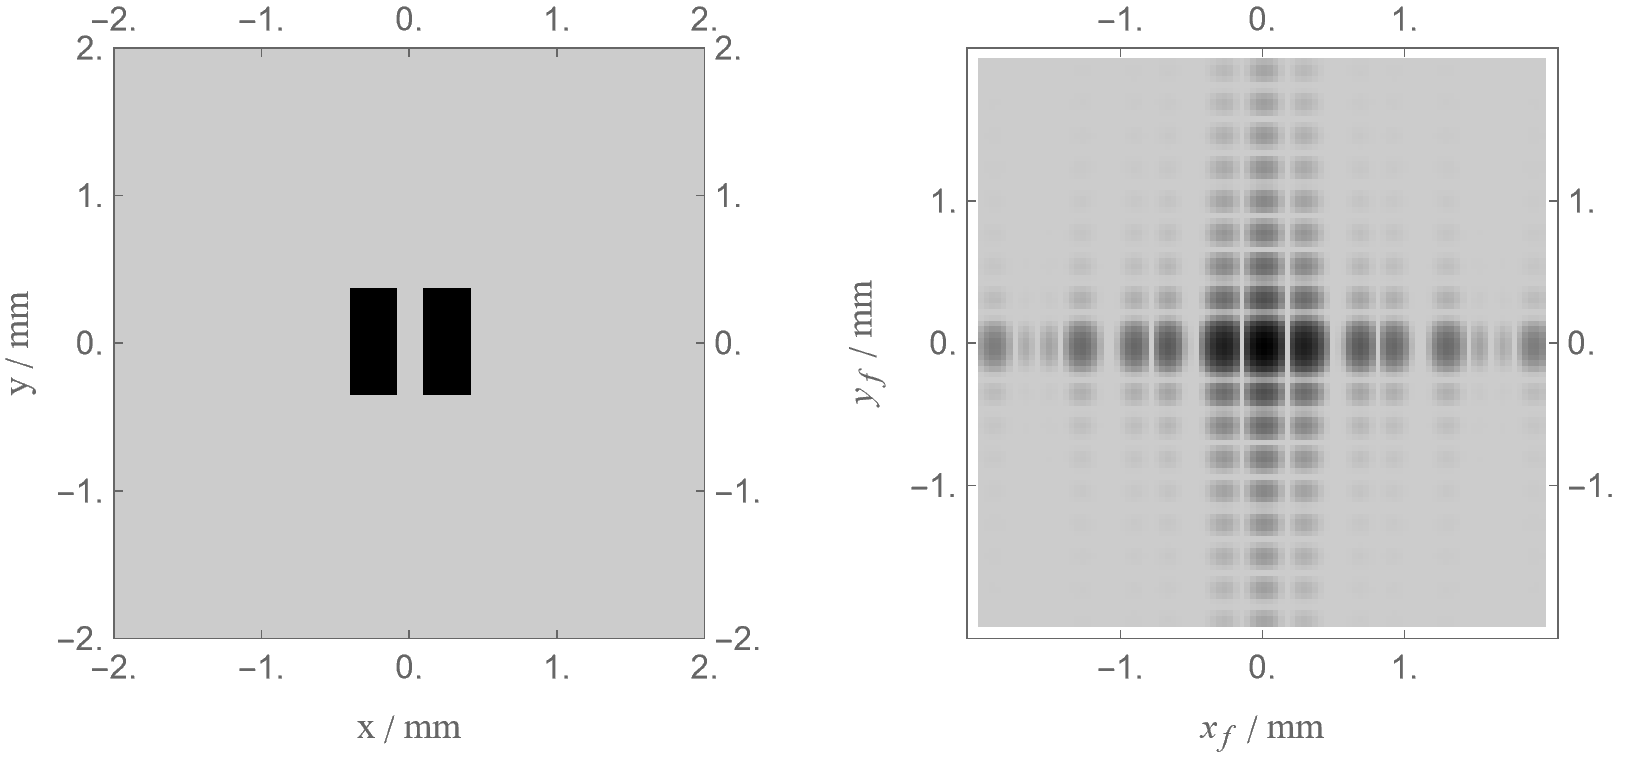
\includegraphics[width=\textwidth]{fourier_optics_4f_fig/double_rectangular_aperture.png}
		\caption{双长方孔}
		\label{fig:object_spectrum_rect_double}
		\label{fig:rect_double}
	\end{subfigure}

	\vspace{0.1cm}
	\begin{subfigure}[b]{0.49\textwidth}
		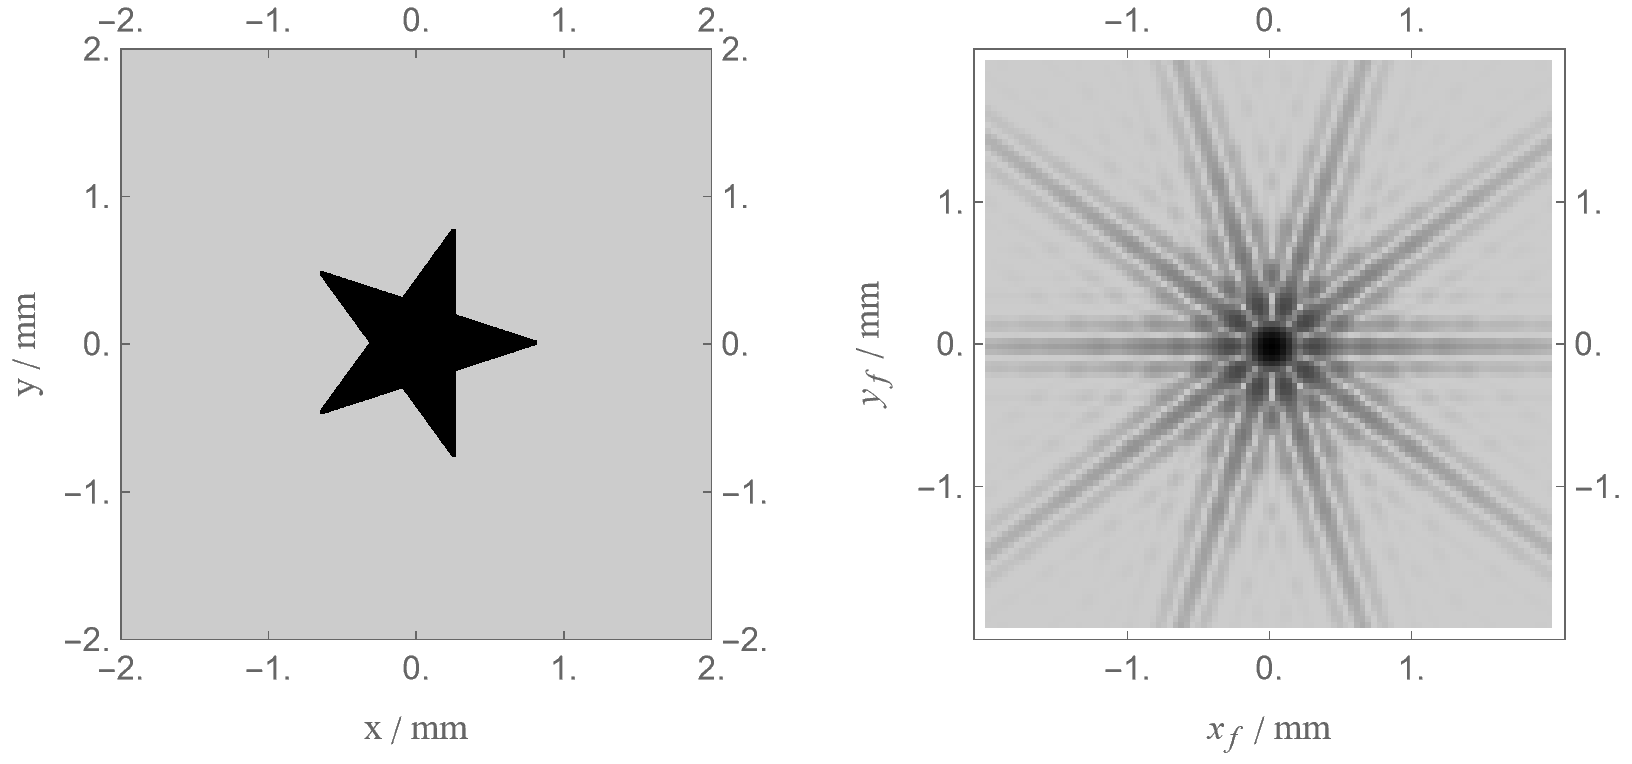
\includegraphics[width=\textwidth]{fourier_optics_4f_fig/pentagram_aperture.png}
		\caption{五角星孔}
		\label{fig:object_spectrum_star}
		\label{fig:star_aperture}
	\end{subfigure}
	\hfill
	\begin{subfigure}[b]{0.49\textwidth}
		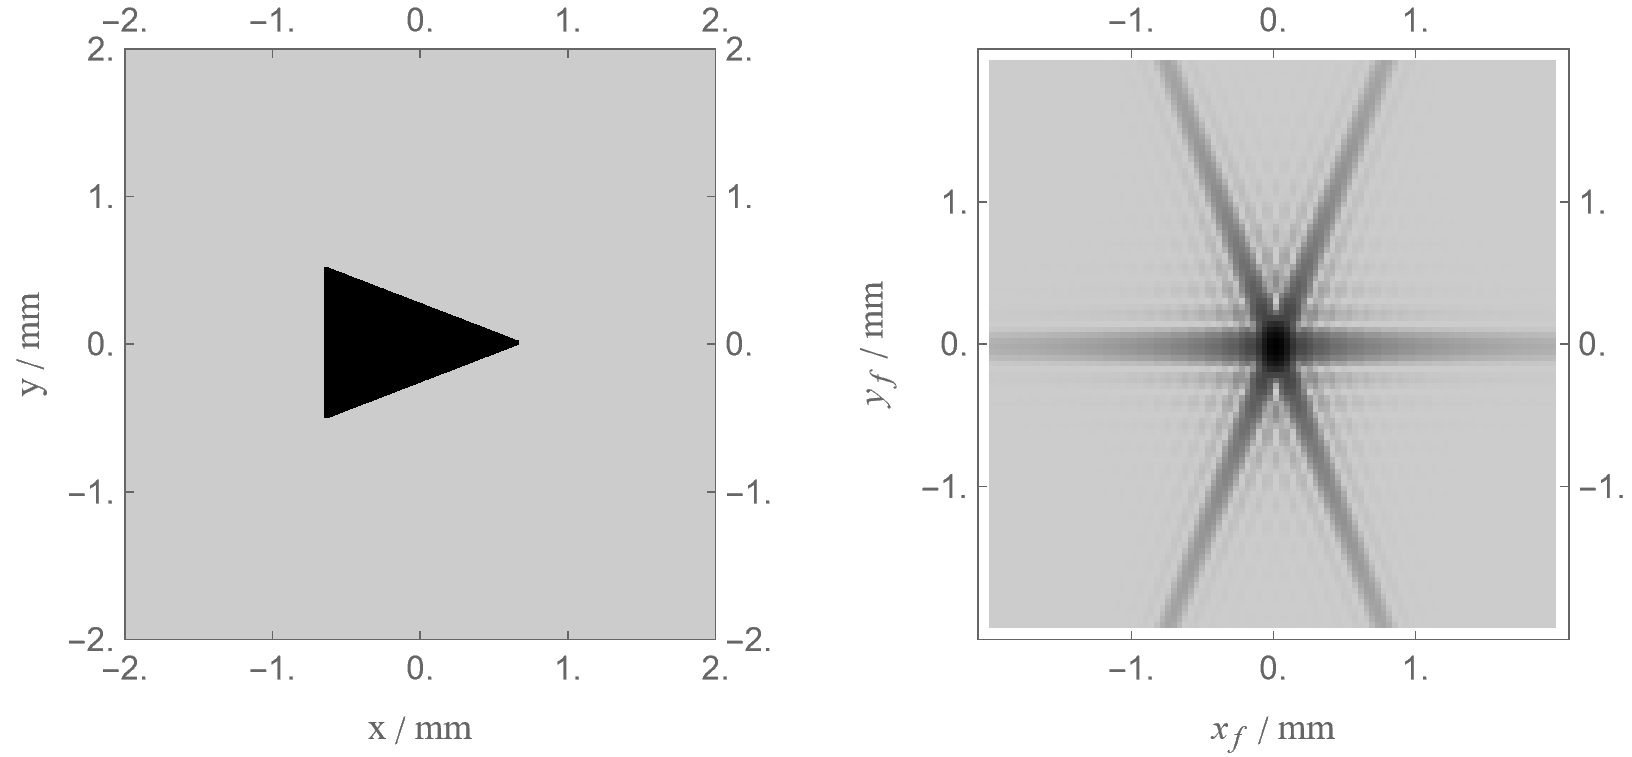
\includegraphics[width=\textwidth]{fourier_optics_4f_fig/isosceles_triangle_aperture.png}
		\caption{等腰三角形孔}
		\label{fig:object_spectrum_triangle}
		\label{fig:isosceles_triangle_aperture}
	\end{subfigure}

	\vspace{0.1cm}
	\begin{subfigure}[b]{0.49\textwidth}
		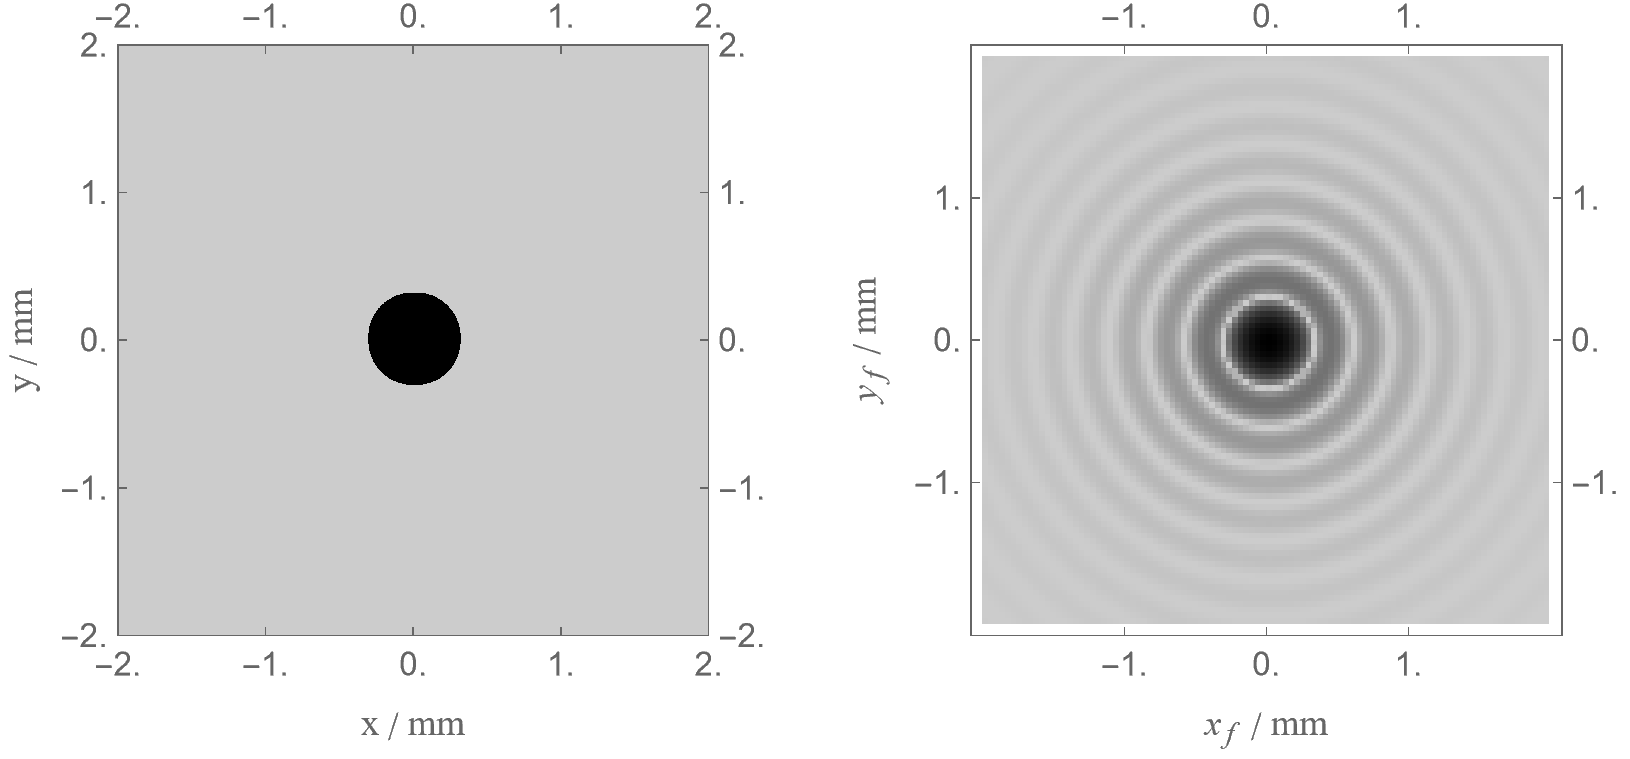
\includegraphics[width=\textwidth]{fourier_optics_4f_fig/single_circular_aperture.png}
		\caption{单圆孔}
		\label{fig:object_spectrum_circle_single}
		\label{fig:circle_single}
	\end{subfigure}
	\hfill
	\begin{subfigure}[b]{0.49\textwidth}
		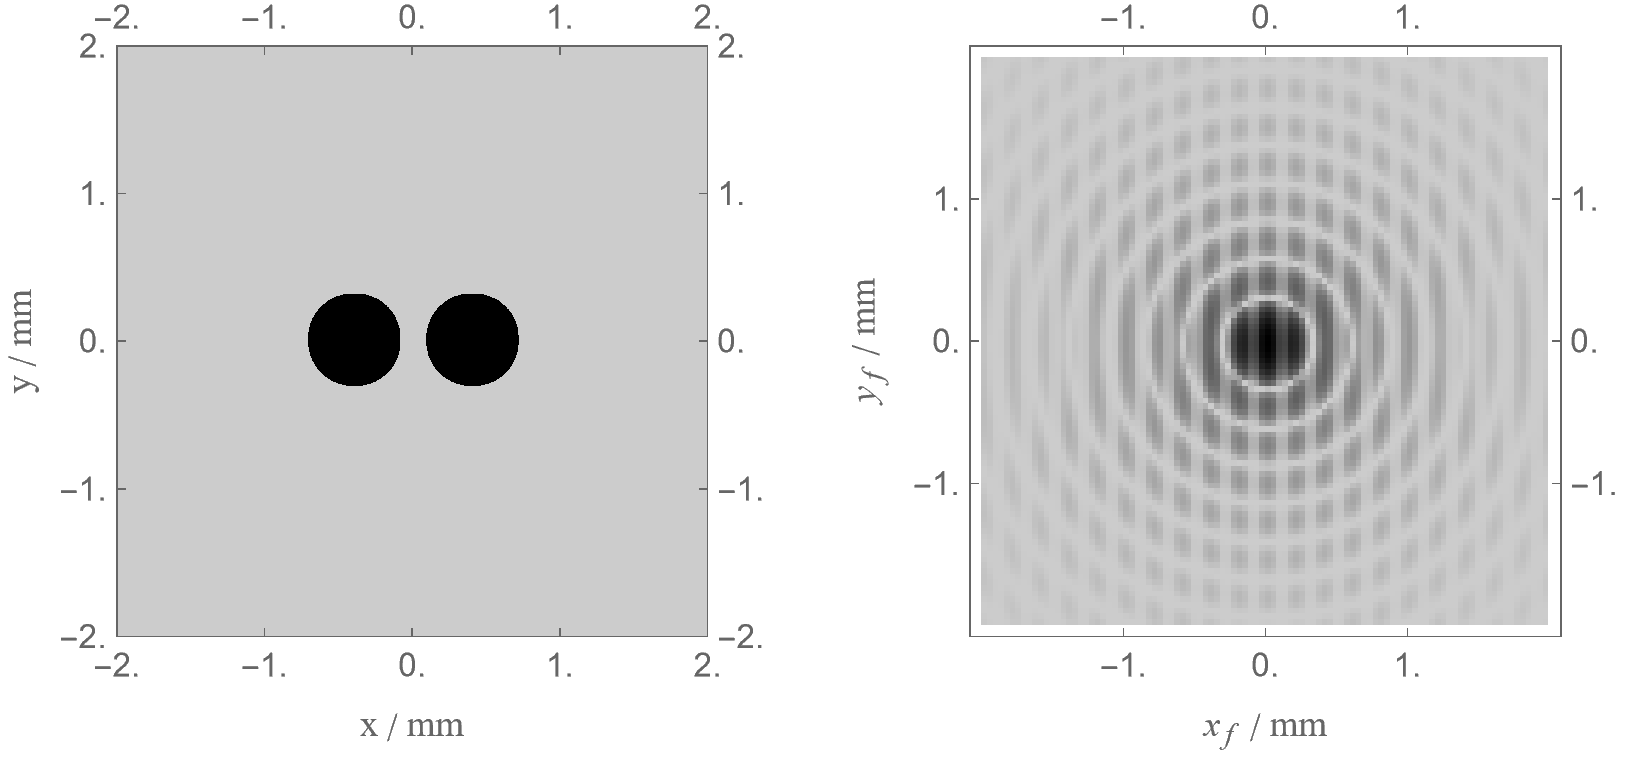
\includegraphics[width=\textwidth]{fourier_optics_4f_fig/double_circular_aperture.png}
		\caption{双圆孔}
		\label{fig:object_spectrum_circle_double}
		\label{fig:circle_double}
	\end{subfigure}

	\vspace{0.1cm}
	\begin{subfigure}[b]{0.49\textwidth}
		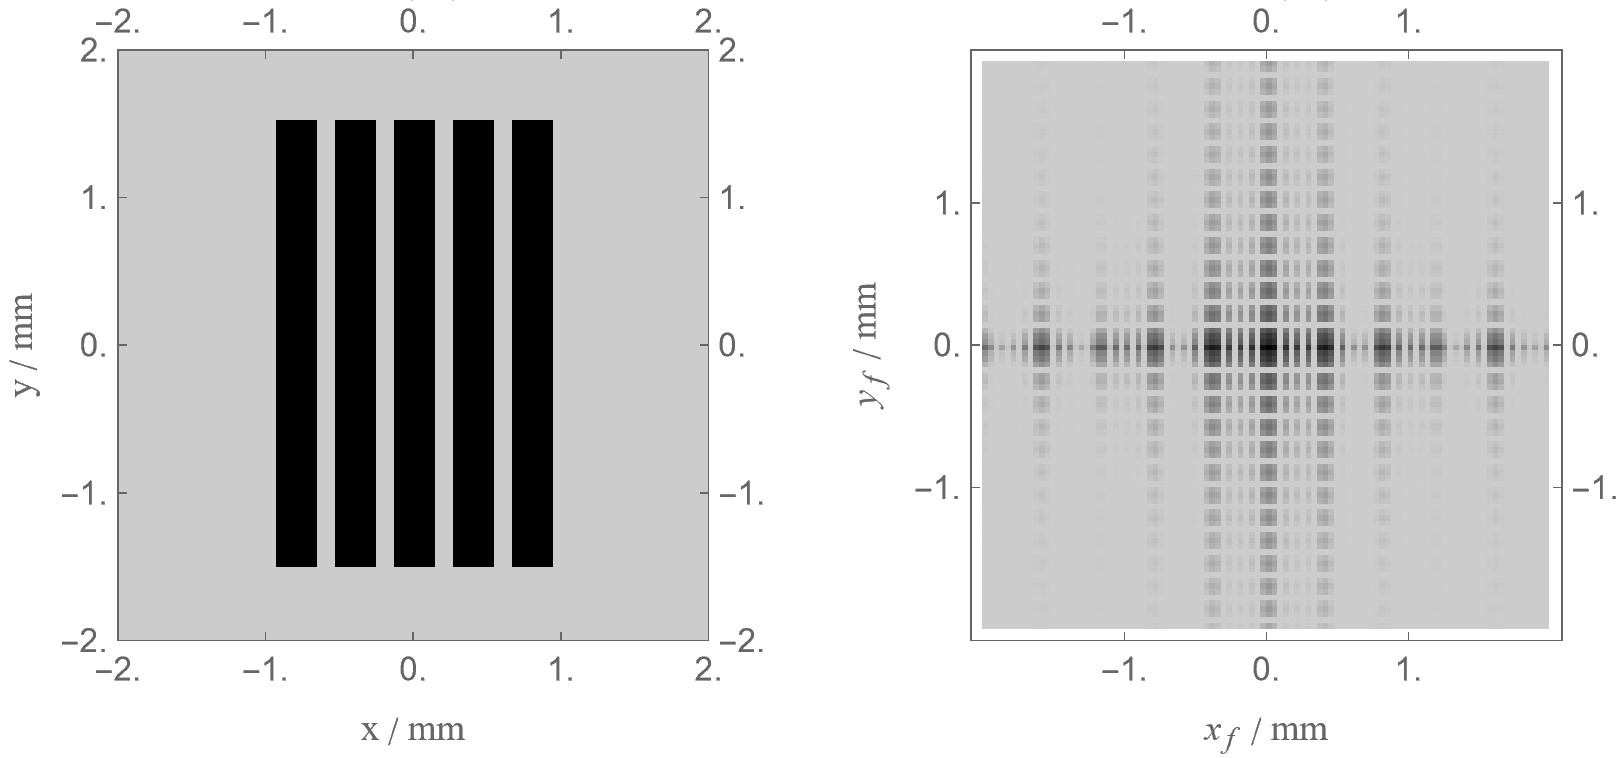
\includegraphics[width=\textwidth]{fourier_optics_4f_fig/five_slits.png}
		\caption{五缝}
		\label{fig:object_spectrum_five_slits}
		\label{fig:five_slits}
	\end{subfigure}
	\hfill
	\begin{subfigure}[b]{0.49\textwidth}
		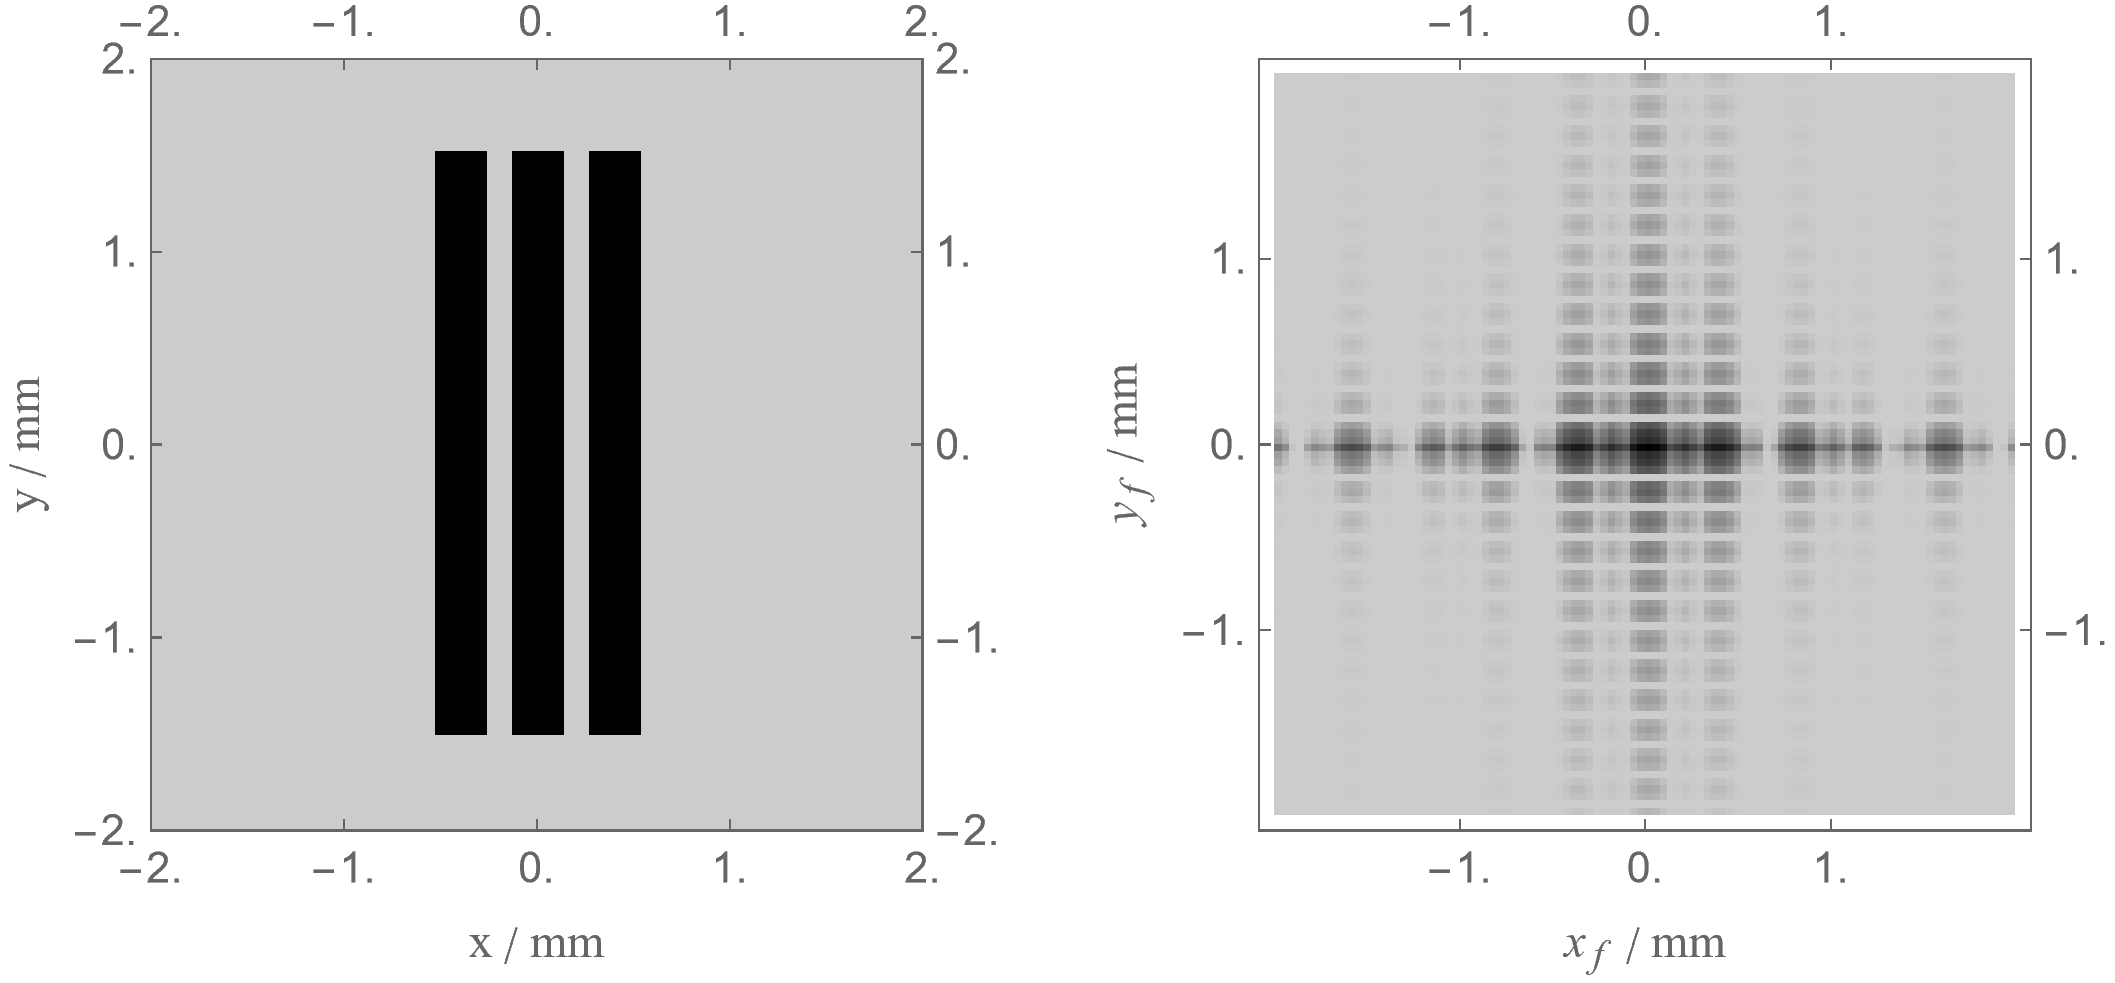
\includegraphics[width=\textwidth]{fourier_optics_4f_fig/three_slits.png}
		\caption{三缝}
		\label{fig:object_spectrum_three_slits}
		\label{fig:three_slits}
	\end{subfigure}

	\vspace{0.1cm}
	\begin{subfigure}[b]{0.49\textwidth}
		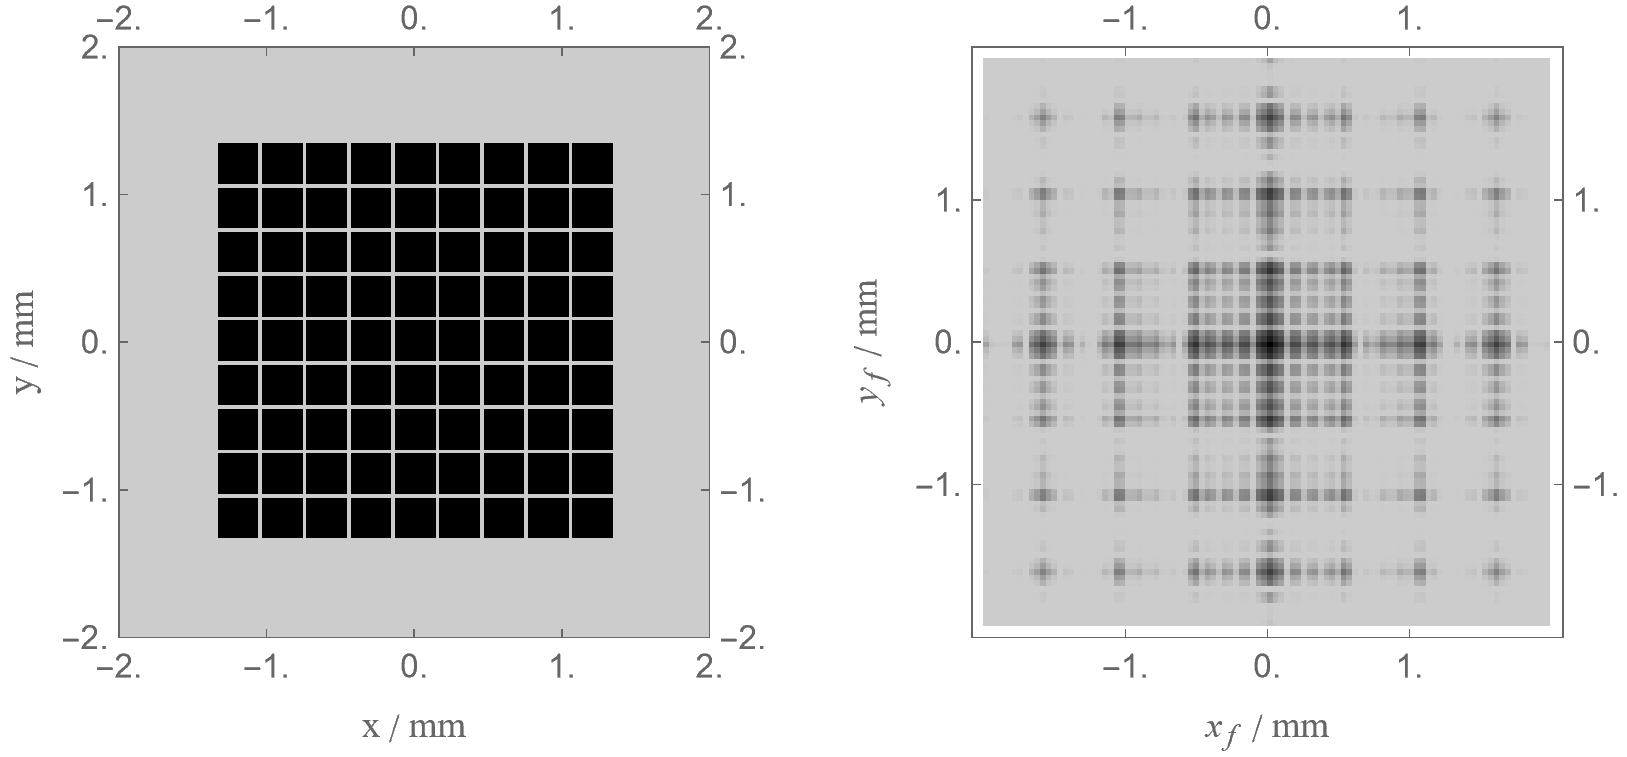
\includegraphics[width=\textwidth]{fourier_optics_4f_fig/cubic_close_packed_square_aperture.png}
		\caption{立方密排方孔}
		\label{fig:object_spectrum_cubic_square}
		\label{fig:cubic_square_aperture}
	\end{subfigure}
	\hfill
	\begin{subfigure}[b]{0.49\textwidth}
		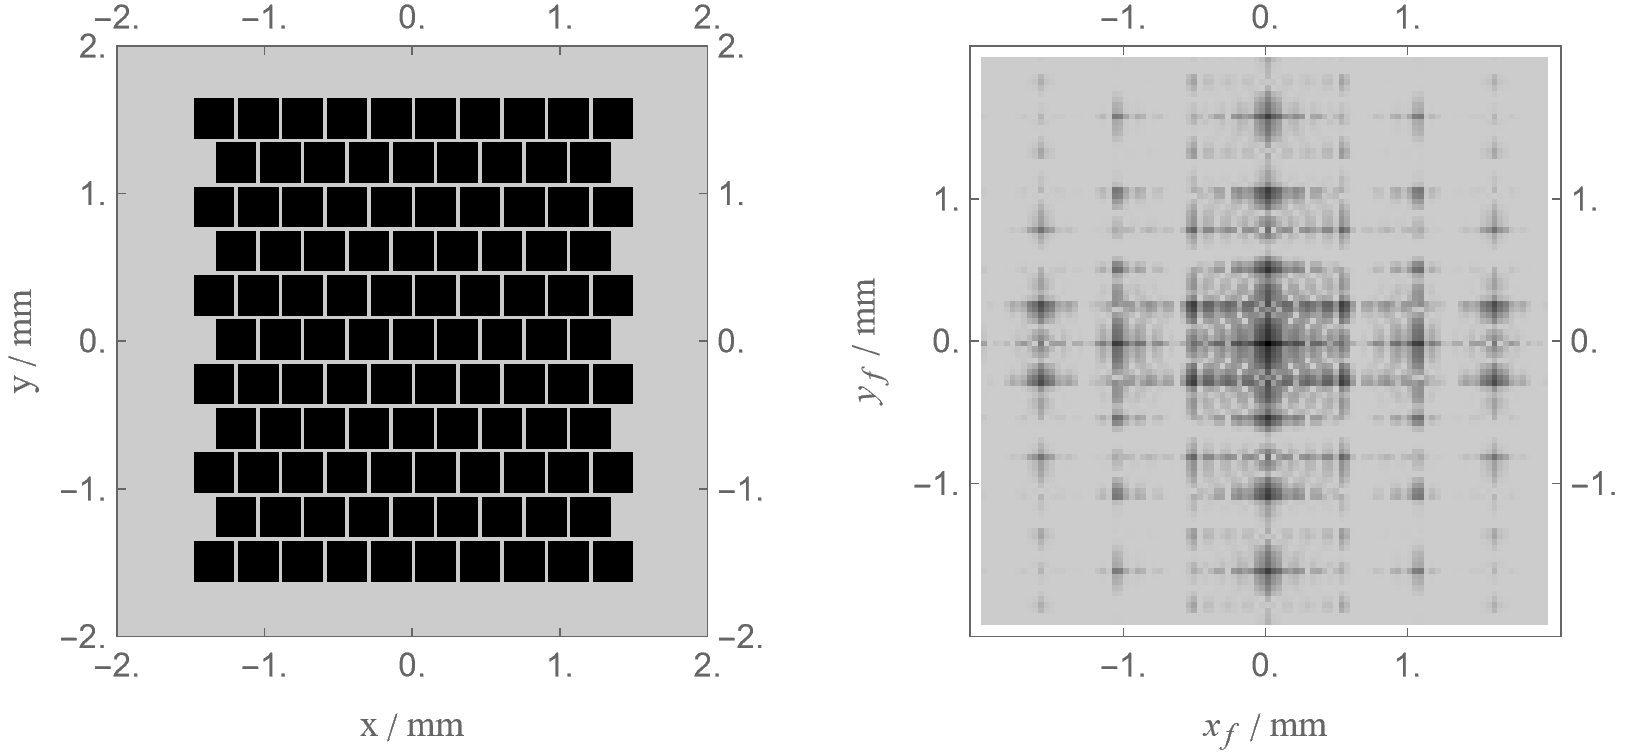
\includegraphics[width=\textwidth]{fourier_optics_4f_fig/hexagonal_close_packed_square_aperture.png}
		\caption{六角密排方孔}
		\label{fig:object_spectrum_hex_square}
		\label{fig:hex_square_aperture}
	\end{subfigure}
\end{figure}
\begin{figure}[htbp]
	\ContinuedFloat

	\begin{subfigure}[b]{0.49\textwidth}
		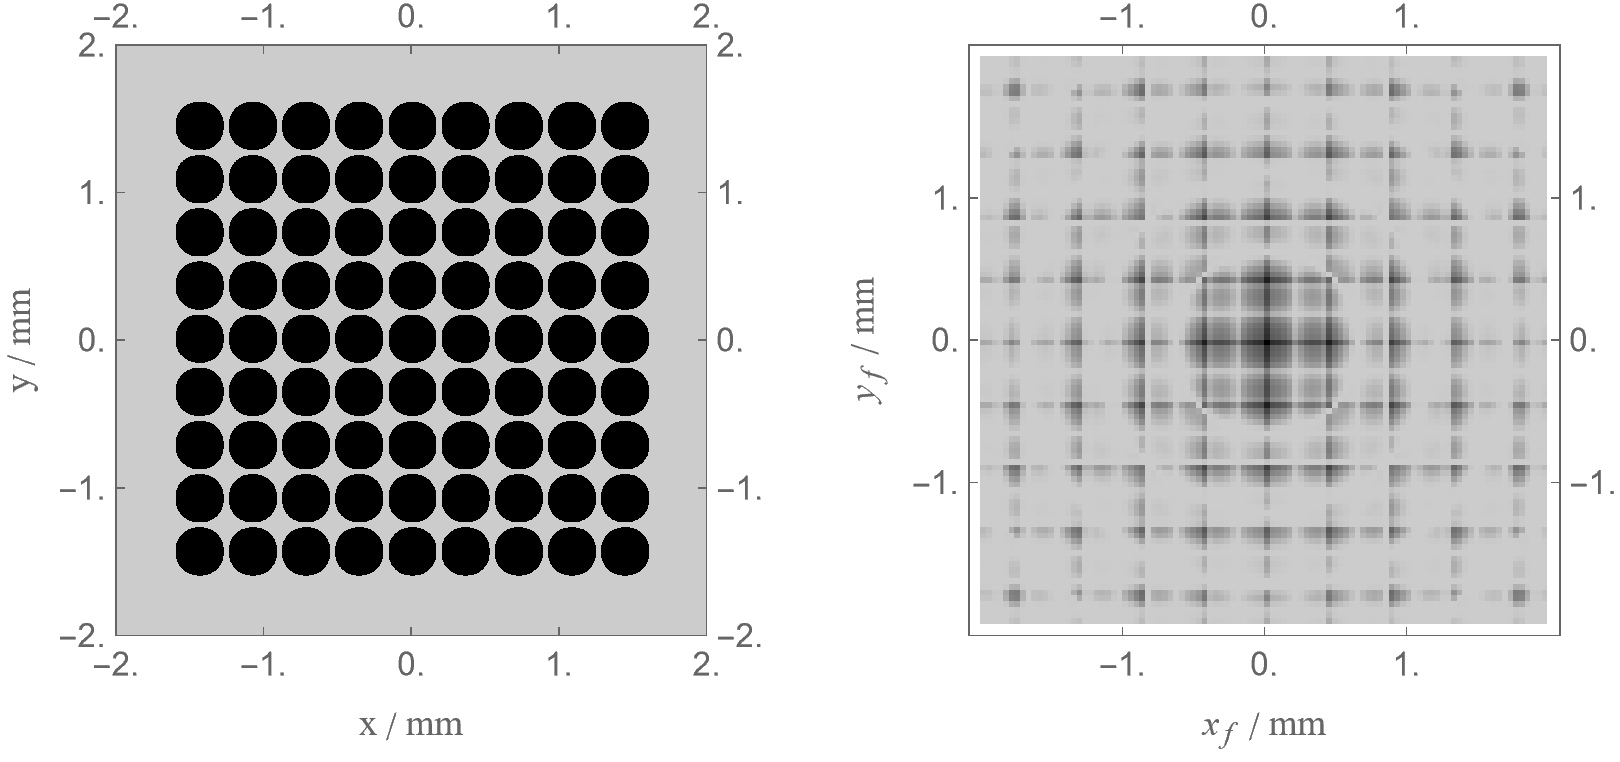
\includegraphics[width=\textwidth]{fourier_optics_4f_fig/cubic_close_packed_circular_aperture.png}
		\caption{立方密排圆孔}
		\label{fig:object_spectrum_cubic_circle}
	\end{subfigure}
	\hfill
	\begin{subfigure}[b]{0.49\textwidth}
		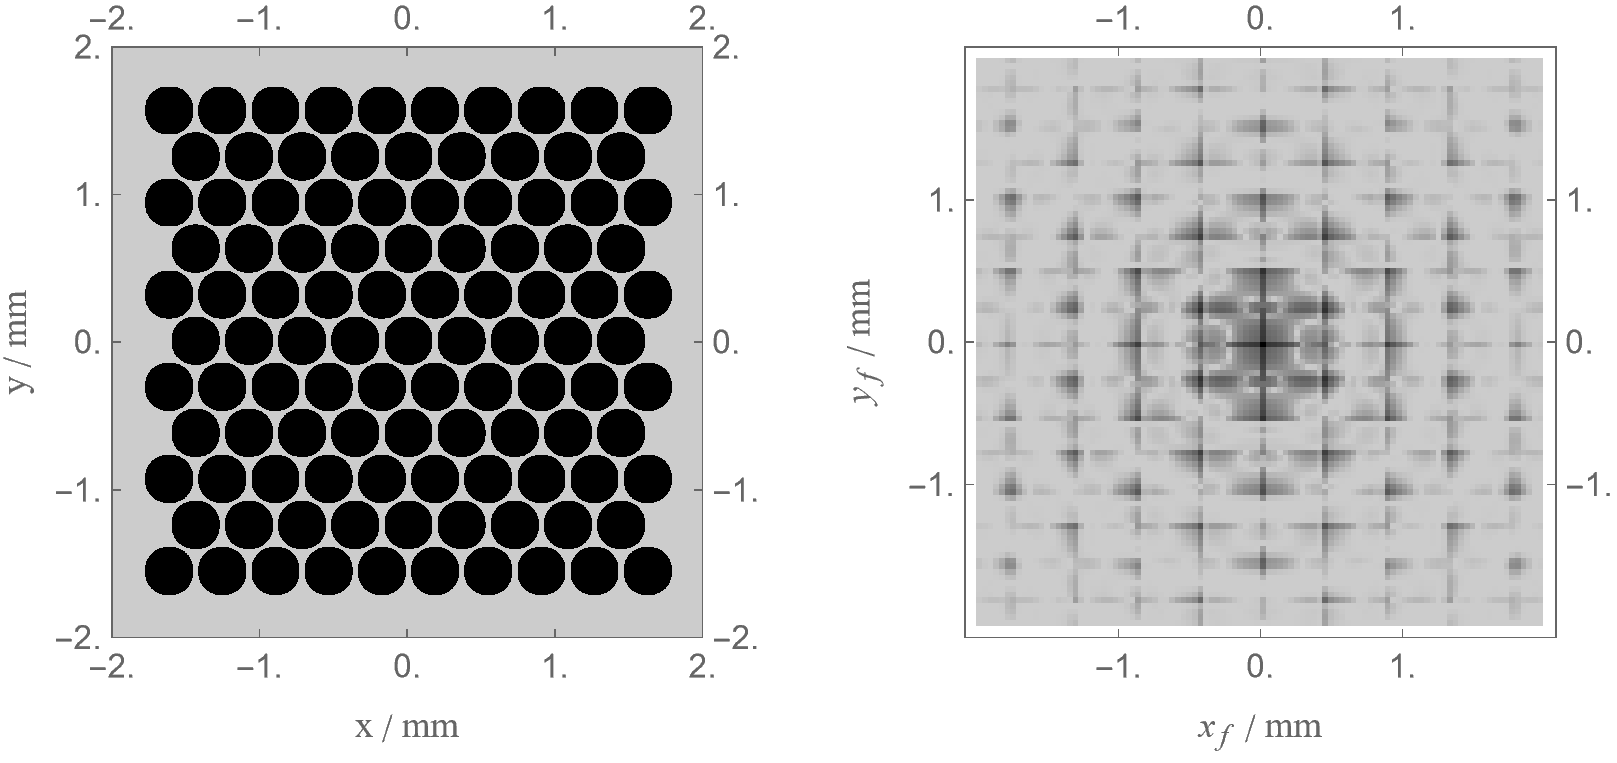
\includegraphics[width=\textwidth]{fourier_optics_4f_fig/hexagonal_close_packed_circular_aperture.png}
		\caption{六角密排圆孔}
		\label{fig:object_spectrum_hex_circle}
	\end{subfigure}

	\vspace{0.1cm}
	\begin{subfigure}[b]{0.49\textwidth}
		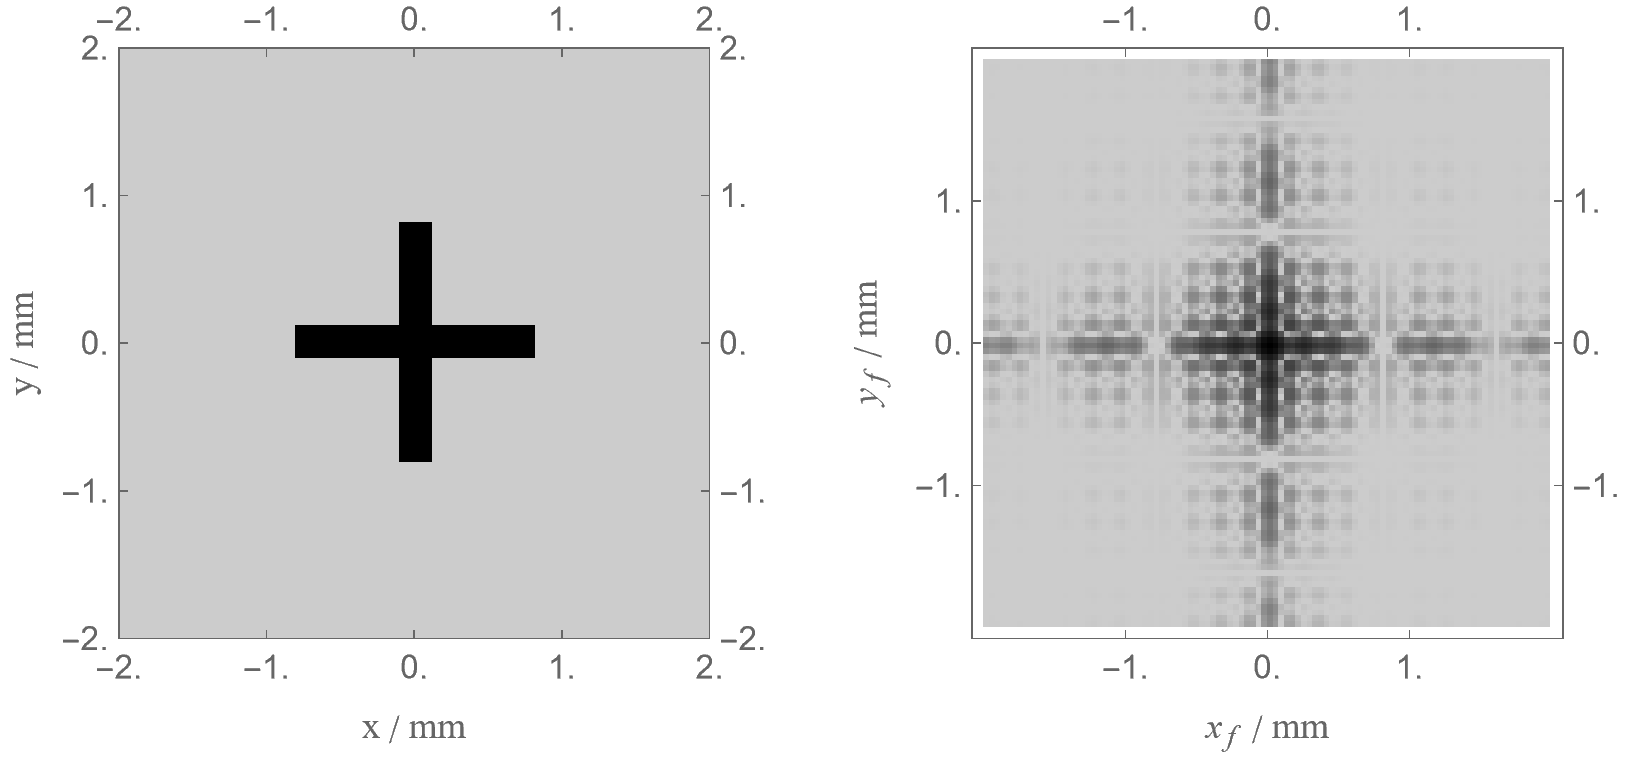
\includegraphics[width=\textwidth]{fourier_optics_4f_fig/cross_aperture.png}
		\caption{“十”字孔}
		\label{fig:object_spectrum_cross}
	\end{subfigure}
	\hfill
	\begin{subfigure}[b]{0.49\textwidth}
		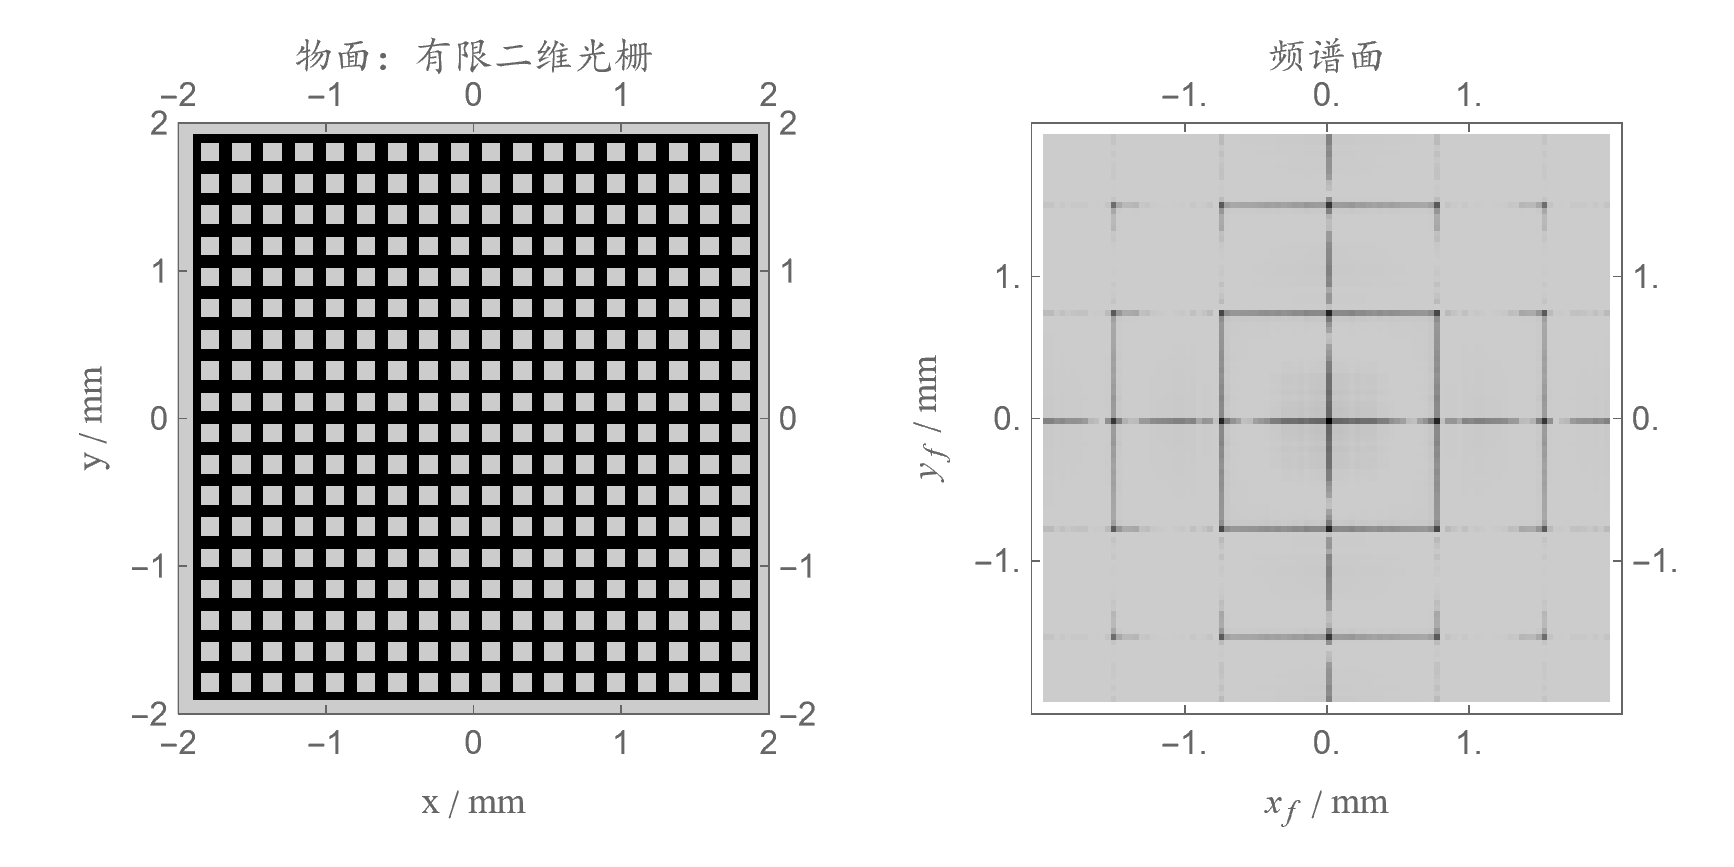
\includegraphics[width=\textwidth]{fourier_optics_4f_fig/two_dimensional_grating.png}
		\caption{二维光栅}
		\label{fig:object_spectrum_2d_grating}
	\end{subfigure}
	\caption{物面及频谱面模拟图}
	\label{fig:object_and_spectrum_plane}
\end{figure}

\section{滤波后的像面振幅分布}

将物面振幅分布与滤波器透射率分布的傅里叶变换做卷积，便得到滤波后的像面振幅分布.
\begin{align*}
	U_P(x, y) =\frac{1}{\lambda f}\iint U_o(\xi, \eta) h(x - \xi, y - \eta) d\xi d\eta.
\end{align*}
其中
\begin{align*}
	h(x, y) = \frac{1}{\lambda f}\iint H(x_f, y_f) e^{i \frac{2\pi}{\lambda f} (x x_f + y y_f)} dx_f dy_f
\end{align*}

\textbf{特别地，考虑一个挡零级斑的小型圆屏滤波器}
\begin{align*}
	H(x_f,y_f)=1-\text{circ}(\frac{\sqrt{x^2+y^2}}{R_H}),\quad h(x,y)=\lambda f \delta(x)\delta(y)-\frac{R_H^2}{\lambda f}A(\frac{2\pi R_H}{\lambda f}\sqrt{x^2+y^2}).
\end{align*}
给出滤波后的像面振幅分布为
\begin{align*}
	U_P(x,y)=U_o(x,y)-\frac{R_H^2}{\lambda^2 f^2}\iint U_o(x-\xi,y-\eta)A(\frac{2\pi R_H}{\lambda f}\sqrt{\xi^2+\eta^2})d\xi d\eta.
\end{align*}

由于滤去了直流成分，图像的亮度会有所减小.未加滤波器时，边界外无光场；而滤去直流后，由于卷积作用可覆盖全空间，故边界外仍有较暗的光场.

最后，用mathematica模拟滤波后的像面.

滤波器的几何尺寸如下：

- 挡零级滤波器是圆心位于原点、半径0.2mm的圆屏.

- 正/斜狭缝滤波器是过原点、与\(y\)轴夹角\(0^\circ/30^\circ\)、宽0.05mm的长方屏.

\begin{figure}[htbp]
	\centering
	\begin{subfigure}[b]{0.24\textwidth}
		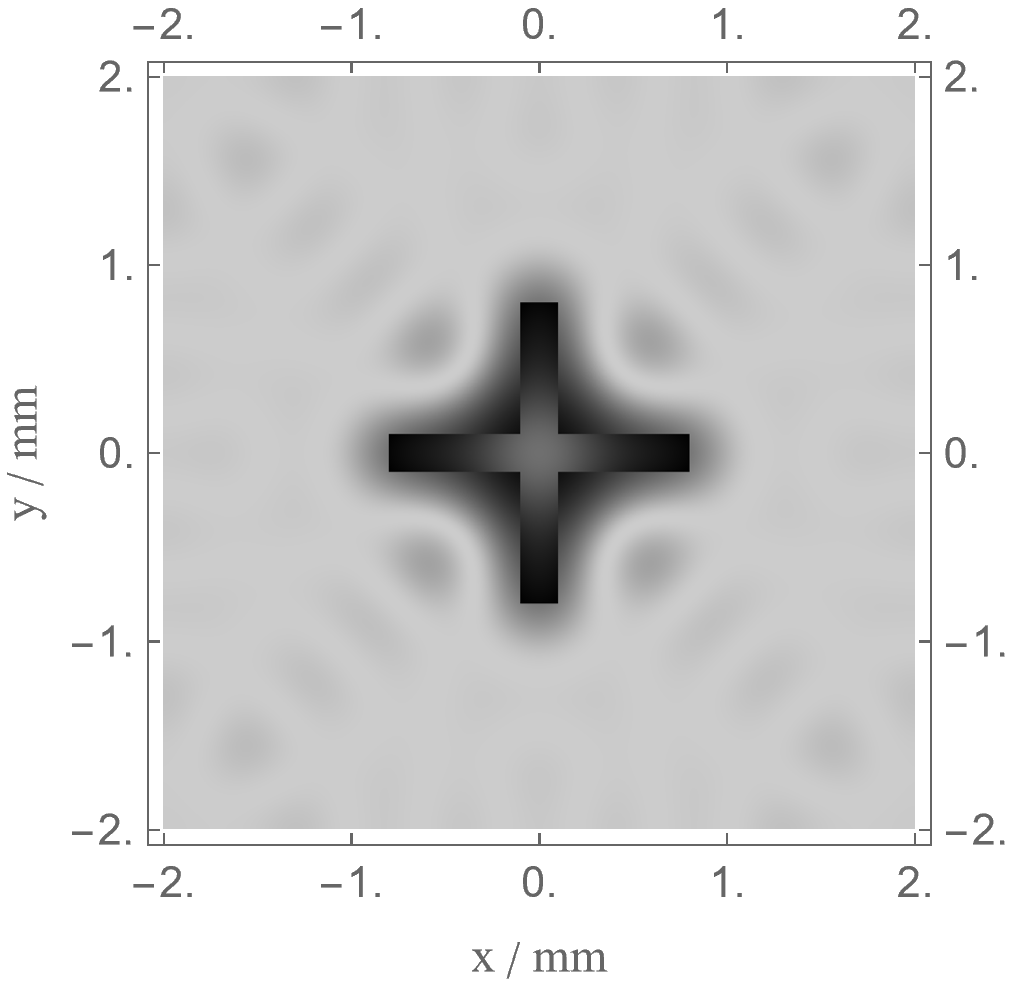
\includegraphics[width=\textwidth]{fourier_optics_4f_fig/cross_aperture_zero_order_blocked.png}
		\caption{“十”字挡零级}
		\label{fig:filtered_image_cross_block_zero}
	\end{subfigure}
	\hfill
	\begin{subfigure}[b]{0.24\textwidth}
		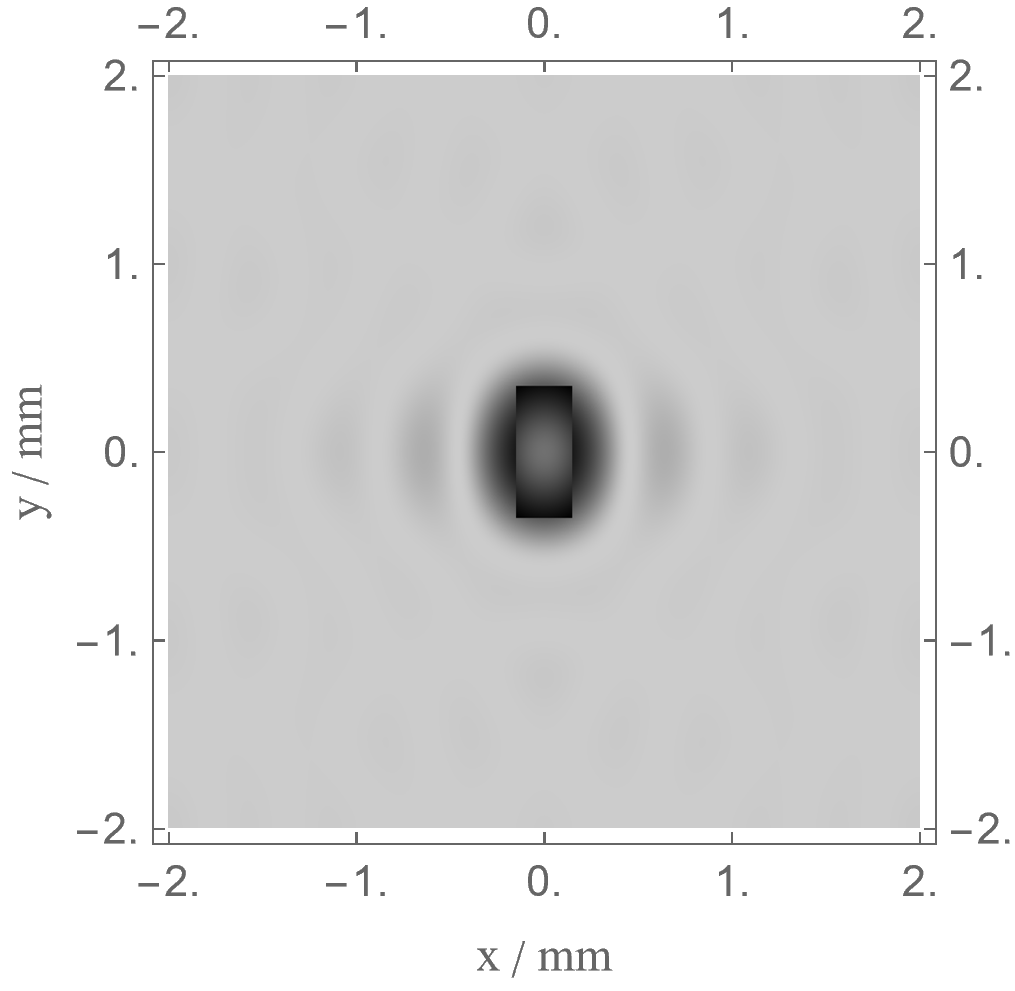
\includegraphics[width=\textwidth]{fourier_optics_4f_fig/single_rectangular_aperture_zero_order_blocked.png}
		\caption{单长方孔挡零级}
		\label{fig:filtered_image_rect_block_zero}
	\end{subfigure}
	\hfill
	\begin{subfigure}[b]{0.24\textwidth}
		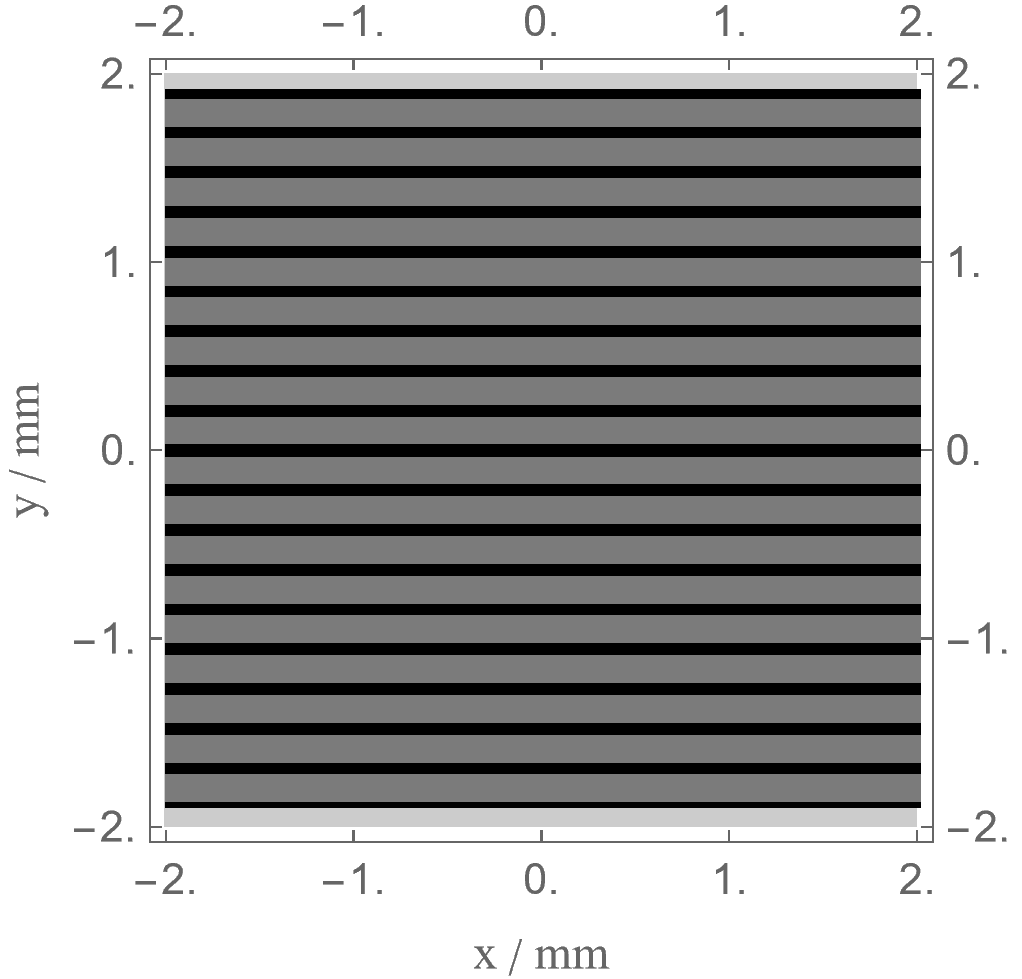
\includegraphics[width=\textwidth]{fourier_optics_4f_fig/two_dimensional_grating_through_vertical_slit.png}
		\caption{二维光栅过正狭缝}
		\label{fig:filtered_image_grating_vertical_slit}
	\end{subfigure}
	\hfill
	\begin{subfigure}[b]{0.24\textwidth}
		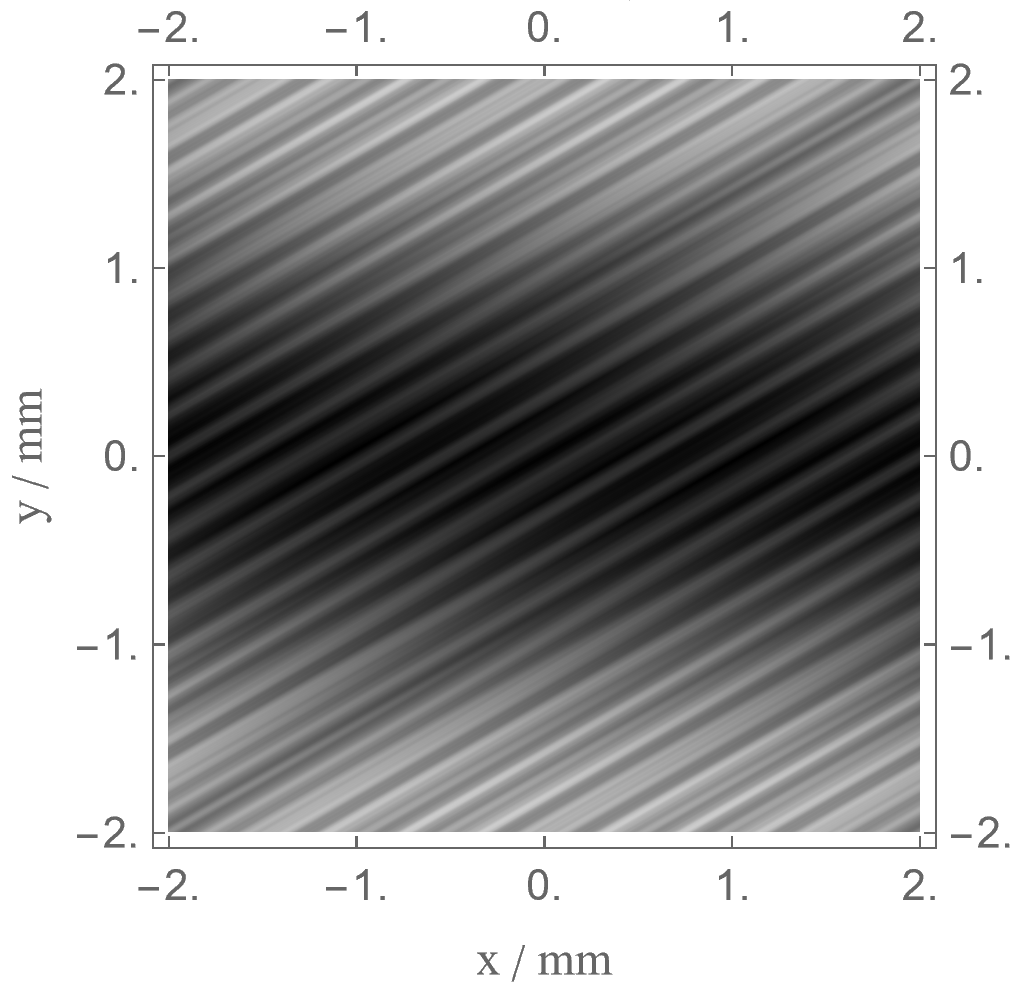
\includegraphics[width=\textwidth]{fourier_optics_4f_fig/two_dimensional_grating_through_oblique_slit.png}
		\caption{二维光栅过斜狭缝}
		\label{fig:filtered_image_grating_tilted_slit}
	\end{subfigure}

	\caption{滤波后像面理论模拟}
	\label{fig:filtered_image_theory}
\end{figure}

\begin{note}
	以上所有图中，灰色代表无光，黑色代表有光，颜色越深、光强越强.具体而言，若入射平面波光强为\(I_o\)，全局最大、最小光强为\(I_{\text{max}},\,I_{\text{min}}\)，则光强为\(I\)处的灰度函数为
	\begin{align*}
		\text{GreyLevel}\left[0.8\left(1-\ln\left(\frac{I_o+I}{I_o+I_{\text{min}}}\right)/\ln\left(\frac{I_o+I_{\text{max}}}{I_o+I_{\text{min}}}\right)\right)\right]
	\end{align*}
	GreyLevel为Mathematica内置的灰度生成函数，参数为零时为纯黑色，参数越大，颜色越浅.
\end{note}


